\documentclass{article}

% ------------------------------------------------------------------
% TMLR submission. Uses the OFFICIAL TMLR style (tmlr.sty, tmlr.bst, fancyhdr.sty
% from github.com/JmlrOrg/tmlr-style-file). Build: tectonic main.tex
% Review version: no package option (double-blind; author block auto-anonymized).
% Camera-ready: change to \usepackage[accepted]{tmlr} and fill in \author + \openreview.
% ------------------------------------------------------------------
\usepackage{times}
\usepackage{tmlr}

\usepackage[utf8]{inputenc}
\usepackage[T1]{fontenc}
\usepackage{hyperref}
\usepackage{url}
\usepackage{booktabs}
\usepackage{amsmath,amssymb,amsfonts}
\usepackage{microtype}
\usepackage{xcolor}
\usepackage{graphicx}
\usepackage{tikz}
\usetikzlibrary{arrows.meta,positioning,fit,backgrounds,calc}
\usepackage{pgfplots}
\pgfplotsset{compat=1.18}

% Figure accent colors (print- and CVD-safe).
\definecolor{figblue}{HTML}{2A78D6}
\definecolor{figorange}{HTML}{EB6834}
\definecolor{figink}{HTML}{0B0B0B}
\definecolor{figmuted}{HTML}{9A9A93}

\newcommand{\kc}{\textsc{kc}}
\newcommand{\regret}{\mathcal{R}}

\title{A Calibrated In-Silico Screen for Corpus Necessity:\\
Constructing the Parametric Ground Truth, and the Misled-Learner Blind Spot}

% Anonymous submission (TMLR).
% In review mode the style prints "Anonymous authors / Paper under double-blind
% review" and ignores this block; fill it in for the [accepted] camera-ready.
\author{Anonymous Author(s)\\Institution\\\texttt{email@example.com}}
% \openreview{\url{https://openreview.net/forum?id=XXXX}}  % camera-ready only

\begin{document}
\maketitle

\begin{abstract}
Before running a human study on a corpus-bounded tutor, a designer wants to know something cheaper
first: does the learner actually \emph{rely} on the curated corpus, or is it coasting on what it
already knows? We present an \emph{in-silico measurement instrument} that answers this as a
behavioral task outcome. The central quantity is \emph{corpus necessity}: ablate a corpus item and
measure the change in a task outcome scored against a reference policy---a with-versus-without
contrast, not an influence score. Our headline move is to make necessity \emph{trustworthy by
constructing its ground truth}: we teach a fact into a model's weights and watch necessity fall as a
\emph{dose-response}. We calibrate the measure in a \emph{simulator-free} fictional-fact
question-answering task scored by an answer checker, where teaching invented facts drives necessity
smoothly to a $\le\!0.05$ floor across a dense 21-point LoRA-scale grid in \emph{five} independent
model families from five labs (Qwen2.5-3B, Phi-3.5-mini, Zephyr-7B, Llama-3.1-8B, OLMo-2-7B; three
seeds each), with each family's transition knee at a different point on the gradient.
A second, \emph{decision}-based domain (a control-regret simulator with a hidden charted hazard) adds a
caution that behavioral-necessity work should heed: a fact taught as prose becomes recallable yet does
\emph{not} move the scored decision---a \emph{knowing\,$\neq$\,doing} gap---unless the knowledge is
\emph{elicited} by reasoning; attempts to \emph{install} the decision by direct fine-tuning instead
yielded a shortcut policy rather than the conditional fact, across three teach-set designs. On this calibrated
measure we build a \emph{corpus diagnosis} that labels each item \emph{relied}, \emph{redundant}
(already known), \emph{unusable} (present but the model fails), or \emph{misled}. The sharp result is
the last: a learner that faithfully follows a \emph{wrong} retrieved rule registers as maximally
reliant---the decision swings hard when the rule is ablated---yet is actively harmed, and standard
necessity and faithfulness metrics, which only ask whether context influenced the output, are blind
to it. Reading necessity as \emph{decision-changes}$\times$\emph{succeeds-with} separates this case
out. We are explicit about scope: every result here is simulation-based mechanism evidence, not
human-subject external validity. This is the pre-human-study screen; the human cohort study is the
pre-registered endpoint it is built to de-risk, and is not a claim of this paper.
\end{abstract}

\section{Introduction}
\label{sec:intro}
A growing body of work builds \emph{corpus-bounded} tutors and assistants: systems that abstain
outside a curated corpus so that, in safety-critical procedural domains, a semantically plausible but
instructionally wrong answer cannot be delivered. A designer who has built such a system faces a
prior question, before any question about learning gains: \emph{does the mechanism work?} Does the
system actually rely on its corpus, and does the corpus actually carry the domain---or is the model
answering from parametric memory and the corpus merely decorative? Answering this by human-subject
study is slow, expensive, and confounded: a null there conflates a broken retrieval mechanism, an
inadequate corpus, an unmotivated cohort, and a dozen other causes.

We argue that the \emph{mechanism} question can be answered cheaply and in silico, and we build the
instrument that does it. The core quantity is \emph{corpus necessity}: remove a corpus item and
measure how much a behavioral task outcome, scored against a reference policy, degrades. This is a
with-versus-without \emph{contrast}, not a measure of whether the context influenced the output. The
difficulty is that a raw necessity reading is confounded---a near-zero value could mean the model
already knew the fact, or that the without-context condition triggered some unrelated heuristic. Our
contribution is to remove that confound \emph{by construction}: we teach a fact into a model's weights
along a graded schedule and show that necessity for that fact falls as a dose-response, giving the
measure a known-groups calibration that influence-based methods structurally lack. On the calibrated
measure we build a \emph{corpus diagnosis} that labels each item relied / redundant / unusable /
\emph{misled}, and its sharpest output is the misled case: a learner faithfully following a wrong
retrieved rule looks maximally reliant yet is harmed, invisible to standard metrics.

Our contribution is a measurement one, scoped as a pre-human-study screen. We make no learning-gains
claim; every result is simulation-based mechanism evidence, and the human cohort study is
pre-registered as the endpoint this screen de-risks, not something we report here. The paper proceeds
as follows: Section~\ref{sec:related} positions the measure against faithfulness and
context-attribution; Section~\ref{sec:instrument} defines the reference-policy instrument and its
construct validity; Section~\ref{sec:necessity} is the headline---necessity read as
different-and-usable, calibrated by the construction dose-response; Section~\ref{sec:diagnosis} turns
the calibrated measure into the corpus diagnosis and the misled result; and
Sections~\ref{sec:limits}--\ref{sec:conclusion} scope and close. Appendices carry the categorical
leakage verdict, a weight-level unlearning cross-check, estimator recovery, and a presence-vs-retrieval
decomposition.

\section{Related work}
\label{sec:related}
\paragraph{Faithfulness, context-attribution, and knowledge conflict.} A large line asks whether a
model uses provided context or parametric memory. Faithfulness metrics score whether an answer is
grounded in the supplied context \citep{ragas2023}; context attribution ablates context sources and
measures the change in output probability to attribute a generation to them \citep{contextcite2024,
priordominance2026}; knowledge-conflict work studies which side wins when context contradicts memory
\citep{knowledgeconflicts2024, faithfulrag2025}; leakage-free benchmarking filters items answerable
with no context \citep{seedrg2026}; and intermediate-step scoring looks beyond the final answer
\citep{cuer2026}. All of these measure whether context \emph{influenced} an output, judged on answer
text, with the corpus \emph{present}. Our delta is on two axes. First, we measure \emph{necessity}, a
with-versus-without contrast---$\mathrm{acc}(\text{with corpus})-\mathrm{acc}(\text{without corpus})$
---rather than influence: a faithfulness score is a function of the \emph{(question, context, answer)}
triple computed with the corpus present, and RAGAS never runs the without-corpus arm, so it is
structurally blind to the quantity---a model that knows a fact and one that does not both score high
with the corpus present. Second, and this is what makes the contrast trustworthy, we \emph{calibrate}
necessity against a constructed weight-level baseline (Section~\ref{sec:necessity}) that these methods
have no analogue for.

\paragraph{The closest relative, and the structural gap.} \textbf{ContextCite} \citep{contextcite2024}
is the nearest method: because it ablates context and measures the change in the response's
log-probability against the model's own baseline, it \emph{partially} tracks necessity. But it requires
open weights and per-token log-probabilities (so it cannot run on the closed-API models our test
covers), attributes text-influence rather than a task outcome, carries no weight-level known-groups
calibration, and yields no relied/redundant/unusable/misled split. The gap common to this whole
strand is that none has a \emph{constructed parametric baseline}: a way to teach a fact into the
weights and confirm the measure responds. That construction (Section~\ref{sec:necessity}) is what lets
us tell a fact the model relied on from one it merely already knew---and, in the misled case, a fact it
faithfully followed off a cliff.

\paragraph{Knowing vs.\ doing.} A separate line finds that knowledge a model holds need not govern its
behavior: facts learned in one form fail to surface in another \citep{reversalcurse2023}, edits leave
messy or mis-scoped ripples \citep{rippleedits2024}, stated reasoning need not reflect the true cause of
an answer \citep{turpin2023cot}, and tool-use exhibits a measured knowing--doing gap
\citep{knowingdoing2026}. We connect this strand to \emph{necessity measurement}: because our instrument
scores a decision, the same gap becomes a validity condition on the measure---a taught fact that is
recallable can leave the scored decision unmoved, so necessity read off a single-shot decision
under-reports it (Section~\ref{sec:necessity}). Unlike \citet{knowingdoing2026}, which reads internal
cognition against tool-call execution, our axis is a counterfactual ablation of a \emph{corpus item}
against a simulator objective, and our construction lets us show the gap closes under elicitation but
not under direct fine-tuning.

\section{The transfer instrument}
\label{sec:instrument}
The necessity measure is a with-versus-without contrast on a \emph{task outcome}; this section defines
that outcome and shows it grades and isolates cleanly, which is what licenses the contrast in
Section~\ref{sec:necessity}.

\paragraph{Task and metric.} The worked domain is COLREG collision avoidance: a power-driven vessel
must choose course and speed to resolve an encounter. We implement a kinematic simulator with an
elliptical ship domain and a Collision Risk Index, and two reference solvers---velocity obstacles
\citep{fiorini1998vo} and simulation-based MPC \citep{johansen2016sbmpc}. For a learner policy $\pi$ on
scenario set $S$ we define the transfer outcome as regret against a reference policy $\pi^\star$,
\begin{equation}
  \regret(\pi) \;=\; \frac{1}{|S|}\sum_{s \in S}\big[\, J(\pi, s) - J(\pi^\star, s)\,\big],
\end{equation}
where $J$ is the per-encounter objective (a weighted sum of a safety-margin barrier, COLREG
compliance penalty, and route deviation; lower is better). We deliberately say ``reference,'' not
``optimal'': VO and SB-MPC are strong near-optimal solvers but not proven globally optimal for the full
nonconvex encounter. The instrument needs only a fixed, reproducible reference that construct validity
shows separates naive from expert behavior; we report which solver is used.

\paragraph{Construct validity and grading.} The instrument must separate good from bad policies before
any necessity claim, and---to be a transfer measure rather than a pass/fail check---the metric must
\emph{grade}, not collapse to two values. Across nine varied encounters (head-on, starboard/port
crossing, overtaking, restricted-visibility geometries), three policies of increasing competence
separate cleanly and continuously on $J$ (Table~\ref{tab:construct}): a naive hold-course policy
(mean $J\approx1765$, clearing $11\%$ of encounters), a velocity-obstacle reference ($J\approx0.70$, all
clear), and SB-MPC ($J\approx0.01$). The objective takes $20$ distinct values in $[0.00, 1995.18]$
over the policy$\times$scenario cells---a graded metric, with the safe regime itself spanning a
continuous $0.00$--$1.27$ range. This is the novice/expert-separation logic of
\citet{vandongen2007lapsim}, applied to a decision/control task.

\begin{table}[t]
\centering
\small
\begin{tabular}{@{}lrrrrr@{}}
\toprule
Policy & mean $J$ & median & min & max & cleared \\
\midrule
naive (hold course) & $1765.44$ & $1988.08$ & $1.08$ & $1995.18$ & $11\%$ \\
VO reference & $0.70$ & $0.58$ & $0.33$ & $1.27$ & $100\%$ \\
SB-MPC reference & $0.01$ & $0.01$ & $0.00$ & $0.03$ & $100\%$ \\
\bottomrule
\end{tabular}
\caption{Construct validity and grading across nine varied encounters. The objective $J$
separates the three competence levels cleanly and takes a continuous range of values
(20 distinct across all cells, $[0.00, 1995.18]$)---a graded transfer metric, not a near-binary check.}
\label{tab:construct}
\end{table}

\paragraph{\kc$\to$single-metric identifiability.} For the diagnosis to attribute a task failure to a
\emph{specific} corpus rule, each knowledge component must govern exactly one metric, so ablating a
\kc\ degrades that metric and no other. This is a design requirement to be verified per instrument,
not a tautology: designing the metrics does not guarantee that ablating one \kc\ leaves the
\emph{others} unchanged---if the objective's terms are entangled, ablation bleeds across metrics.
Identifiability is the empirically-checked absence of that bleed. On a discrete procedural domain
(a roadside tire change) the verification is clean (Table~\ref{tab:ident}): each ablation degrades only
its governed metric, maximum off-diagonal change $0.0000$. Because the property holds on both a
continuous-control and a discrete-procedural instrument, it is a general measurement-design property,
not a COLREG artifact. Estimator-recovery and calibration on synthetic data appear in
Appendix~\ref{app:recovery}.

\begin{table}[t]
\centering
\small
\begin{tabular}{@{}lcccc@{}}
\toprule
ablated \kc\ $\downarrow$ / metric $\rightarrow$ & safety & core & sequencing & finishing \\
\midrule
safety      & $\mathbf{-1.00}$ & $0.00$ & $0.00$ & $0.00$ \\
core steps  & $0.00$ & $\mathbf{-1.00}$ & $0.00$ & $0.00$ \\
sequencing  & $0.00$ & $0.00$ & $\mathbf{-0.22}$ & $0.00$ \\
finishing   & $0.00$ & $0.00$ & $0.00$ & $\mathbf{-1.00}$ \\
\bottomrule
\end{tabular}
\caption{\kc$\to$single-metric identifiability (procedural domain). Change in each metric after
ablating each knowledge component. The diagonal (bold) is the intended governed metric; every
off-diagonal cell is $0.00$ (max $|\Delta|=0.0000$)---ablation does not bleed across metrics.}
\label{tab:ident}
\end{table}

\section{Necessity, calibrated by construction}
\label{sec:necessity}
This is the headline. We first fix how necessity should be \emph{read} off the instrument, then make
the reading trustworthy by constructing its ground truth.

\paragraph{Necessity as \emph{different and better}.} Ablate a corpus item and compare the run against
the with-corpus run on two observables (Figure~\ref{fig:diffbetter}): does the \emph{decision} change
(\textbf{different}), and does the learner \emph{succeed with} the item present (\textbf{usable})? An
item is \textbf{relied on} only when the corpus changes the decision \emph{for the better}---removing
it flips a succeeding call into a failing one. Reading necessity as ``the corpus changed the call, and
it helped'' is stronger than the subtractive ``nothing broke when we removed it,'' and, crucially, the
two-observable reading is what will separate genuine reliance from the \emph{misled} case in
Section~\ref{sec:diagnosis}: a corpus item can change the decision hard (high raw necessity) while the
learner still \emph{fails} with it present, which the subtractive test cannot see. This reading is
computed off the graded regret instrument itself, not a decoupled side-metric.

\begin{figure}[t]
\centering
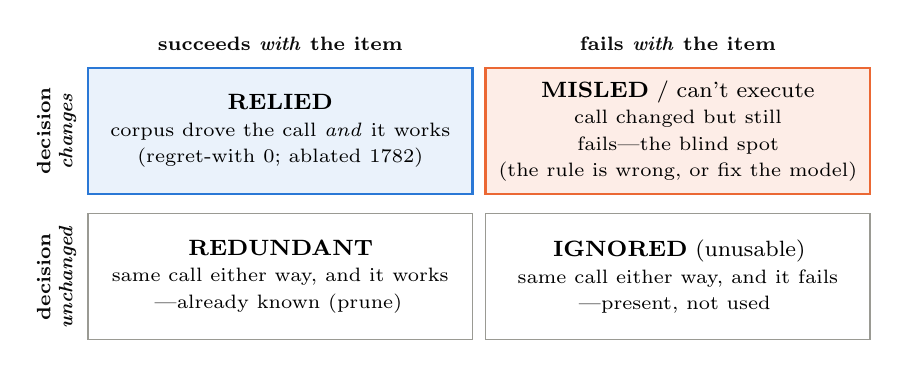
\begin{tikzpicture}[font=\footnotesize,
  cell/.style={draw=figmuted, line width=0.5pt, text width=46mm, minimum height=16mm,
               align=center, inner sep=4pt, outer sep=0pt},
  relied/.style={cell, fill=figblue!10, draw=figblue, line width=1pt},
  sharp/.style={cell, fill=figorange!12, draw=figorange, line width=1pt},
  lbl/.style={font=\scriptsize\bfseries, text=figink}]
\node[relied]                 (tl) at (0,0)     {\textbf{RELIED}\\{\scriptsize corpus drove the call \emph{and} it works}\\{\scriptsize (regret-with $0$; ablated $1782$)}};
\node[sharp]                  (tr) at (5.05,0)  {\textbf{MISLED} / can't execute\\{\scriptsize call changed but still fails---the blind spot}\\{\scriptsize (the rule is wrong, or fix the model)}};
\node[cell]                   (bl) at (0,-1.85) {\textbf{REDUNDANT}\\{\scriptsize same call either way, and it works}\\{\scriptsize ---already known (prune)}};
\node[cell]                   (br) at (5.05,-1.85) {\textbf{IGNORED} (unusable)\\{\scriptsize same call either way, and it fails}\\{\scriptsize ---present, not used}};
\node[lbl, above=1mm of tl.north] {succeeds \emph{with} the item};
\node[lbl, above=1mm of tr.north] {fails \emph{with} the item};
\node[lbl, rotate=90, anchor=center, align=center] at ($(tl.west)+(-4mm,0)$) {decision\\\emph{changes}};
\node[lbl, rotate=90, anchor=center, align=center] at ($(bl.west)+(-4mm,0)$) {decision\\\emph{unchanged}};
\end{tikzpicture}
\caption{Necessity read as \emph{different}$\times$\emph{usable}: ablate an item and ask whether the
\emph{decision} changes (rows) and whether the learner \emph{succeeds with} it present (columns).
Blue (top-left) is the only \textbf{relied} cell---the corpus changed the call, for the better.
Orange (top-right) is the \emph{misled}/can't-execute case: maximal raw necessity yet a harmful
outcome, invisible to a subtractive ``did removing it hurt?'' test---the blind spot this measure is
built to expose. A coarser categorical verdict is deferred to Appendix~\ref{app:verdict}.}
\label{fig:diffbetter}
\end{figure}

\paragraph{Why the reading needs calibration.} The necessity test infers a fact about a model's
\emph{weights} from a change in the \emph{prompt}: ablate an item, and if the governed outcome does not
move, the model did not need it. The sharpest objection is that context removal is not weight-level
knowledge change, so a small necessity could be a no-context heuristic in disguise, or a large
necessity could reflect a fact the model happens not to know for reasons we did not control. We close
this \emph{by construction}: if teaching a fact into the weights drives necessity for that fact down as
a dose-response, then a near-zero reading is evidence the model already knew the item, and the measure
is a non-confounded, known-groups quantity. We build models along a gradient from fact-naive to
fact-knowing by teaching a target fact into the weights (LoRA SFT), moving the gradient by two
independent knobs---the LoRA scale $\alpha$ (one adapter, evaluated at $\alpha\in[0,1]$) and genuine
training checkpoints---so that a result reproducing under an independent axis rules out a
gradient-method artifact. We establish the calibration in a simulator-free QA domain---where the
$\alpha$ sweep replicates across five model families---then use a decision-based domain, where the flat
result holds under both knobs, to surface a limit the calibration alone would hide.

\paragraph{The calibration: simulator-free fictional-fact QA.} We invent facts about fictional entities
(research outposts and their attributes) that no model can have memorized, and score answers with a
programmatic checker---no simulator, no reference policy. Because the facts are fictional, a competent
model is necessarily corpus-bound at baseline, and because there are many \emph{independent} facts,
partial teaching learns a fraction of them, so the aggregate necessity is \emph{graded}. Teaching the
facts into \emph{five} independent model families---five distinct pretraining lineages, three seeds
each, in a single clean run---drives mean necessity smoothly down a dense 21-point LoRA-$\alpha$ grid
($0$ to $1$ in steps of $0.05$) to a $\le\!0.05$ floor in every family (Figure~\ref{fig:factqa_dose};
a table subset in Table~\ref{tab:dose}). Each family's transition knee sits at a \emph{different}
$\alpha$ (Zephyr-7B $\approx\!0.30$, Llama-3.1-8B $\approx\!0.35$, OLMo-2-7B $\approx\!0.45$,
Qwen2.5-3B $\approx\!0.50$, Phi-3.5-mini $\approx\!0.65$), so five architectures give the same
collapse on their own schedules---ruling out a single-model or single-schedule artifact---and the
graded floor near zero is what a near-zero reading on the real instrument is calibrated against. Every
seed is monotone through its transition; deviations are confined to the endpoints---$\le\!0.04$
per-step wiggles at the near-zero floor, and two families (Llama $0.96$, OLMo $0.95$) starting
slightly below $1.00$ because the base model guesses a probe correctly closed-book, consistently
across seeds, before reaching $\approx\!1.00$ by $\alpha\!\approx\!0.15$. An earlier independent run
(different adapters, coarser grid) reproduces the shared points almost exactly (Qwen $0.47$ vs.\
$0.47$, Phi $0.93$ vs.\ $0.93$, Zephyr $0.09$ vs.\ $0.09$ at $\alpha{=}0.5$)---the same instrument
reading twice. This is the known-groups calibration, in a domain we did not
build a simulator for---answering the objection that the measure is an artifact of one hand-built
environment. (Necessity here is measured closed-book: the without-corpus condition permits parametric
answering, so taught knowledge surfaces rather than being suppressed by a strict ``answer only from the
provided facts'' instruction.)

\paragraph{A decision-domain caution: knowing\,$\neq$\,doing.} The calibration teaches and scores in the
\emph{same} channel---a fact, queried as a fact. A behavioral instrument scores a \emph{decision}, and
there the two can come apart, so we probe the decision domain directly with a corpus-only charted
hazard (a danger scored by the objective barrier but not shown in the prompt, knowable only from the
corpus) taught into a Qwen2.5-3B model \emph{as prose}. The fact becomes \emph{recallable}---free-text
recall of the avoiding action rises from $0.00$ to $0.78$---yet the scored maneuver \emph{does not
move}: $\regret$-necessity is flat ($\approx\!667$ at both the naive and taught ends), and stays flat
across both the LoRA-scale gradient and a genuine partial-training checkpoint sweep (three seeds; one
seed shows a transient turn only at deep intermediate checkpoints, and the fully-taught adapter returns
to $667$---an instability, not a reached decision). The fact is in
the weights but does not reach the decision: a \emph{knowing\,$\neq$\,doing} gap, a behavioral cousin of
the reversal curse \citep{reversalcurse2023} and of the knowing--doing gap reported for tool use
\citep{knowingdoing2026}. Two interventions localize it (Figure~\ref{fig:knowdo}). \emph{Eliciting} the
knowledge by reason-then-decide prompting closes the gap---necessity falls to $\approx\!0.3$, while a
naive-model reasoning control still grounds, so it is the taught knowledge being surfaced, not reasoning
alone.
\emph{Installing} the decision directly by fine-tuning on the scored format does not: across
positive-only, contrastive, and surface-debiased teach sets the model learns a blanket or shortcut
policy---confabulating the hazard at every location, an instance of unfaithful
reasoning~\citep{turpin2023cot} and of mis-scoped knowledge editing~\citep{rippleedits2024}---never the
conditional fact (Appendix~\ref{app:unlearning} reports the parallel weight-level
\emph{says\,$\neq$\,does} dissociation from unlearning). The lesson for the measure: on a decision
objective, whether a taught fact ``counts'' depends on whether it is \emph{elicited}, so necessity read
off a single-shot decision can under-report knowledge the model in fact holds---a validity caveat we
return to in Section~\ref{sec:limits}.

\begin{figure}[t]
\centering
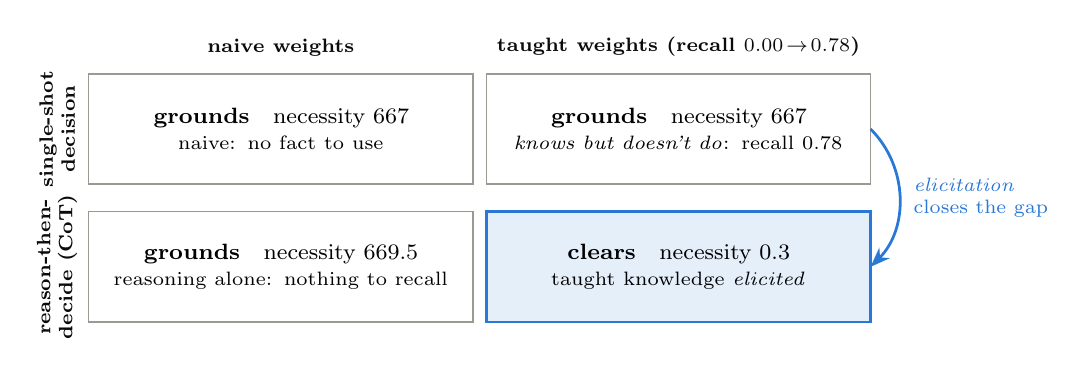
\begin{tikzpicture}[font=\footnotesize,
  cell/.style={draw=figmuted, line width=0.5pt, text width=46mm, minimum height=14mm,
               align=center, inner sep=4pt, outer sep=0pt},
  clears/.style={cell, fill=figblue!12, draw=figblue, line width=1pt},
  lbl/.style={font=\scriptsize\bfseries, text=figink}]
\node[cell]   (tl) at (0,0)      {\textbf{grounds}\quad necessity $667$\\{\scriptsize naive: no fact to use}};
\node[cell]   (tr) at (5.05,0)   {\textbf{grounds}\quad necessity $667$\\{\scriptsize \emph{knows but doesn't do}: recall $0.78$}};
\node[cell]   (bl) at (0,-1.75)  {\textbf{grounds}\quad necessity $669.5$\\{\scriptsize reasoning alone: nothing to recall}};
\node[clears] (br) at (5.05,-1.75) {\textbf{clears}\quad necessity $0.3$\\{\scriptsize taught knowledge \emph{elicited}}};
\node[lbl, above=1mm of tl.north] {naive weights};
\node[lbl, above=1mm of tr.north] {taught weights (recall $0.00\!\to\!0.78$)};
\node[lbl, rotate=90, anchor=center, align=center] at ($(tl.west)+(-4mm,0)$) {single-shot\\decision};
\node[lbl, rotate=90, anchor=center, align=center] at ($(bl.west)+(-4mm,0)$) {reason-then-\\decide (CoT)};
\draw[-{Stealth[length=2.5mm]}, figblue, line width=1pt]
  (tr.east) to[bend left=45]
  node[right=0.5mm, align=left, font=\scriptsize, text=figblue]
  {\emph{elicitation}\\closes the gap} (br.east);
\end{tikzpicture}
\caption{The knowing\,$\neq$\,doing gap and its bridge, on the hazard decision ($\regret$-necessity;
lower $=$ clears without the corpus). The taught fact is recallable (top-right, recall $0.00\!\to\!0.78$)
yet leaves the single-shot decision unmoved (top row, flat $667$). Only \emph{reason-then-decide on the
taught model} clears (bottom-right, $0.3$, blue); reasoning on the naive model does not
(bottom-left), so the turn is the taught knowledge being elicited, not reasoning alone---the action
needs \emph{both} the knowledge \emph{and} the elicitation (arrow). Installing the decision directly by
fine-tuning does not reproduce this: it yields a blanket/confabulated policy
(\texttt{decision-teach-arc.md}), not the conditional fact.}
\label{fig:knowdo}
\end{figure}

\begin{figure}[t]
\centering
\IfFileExists{figures/factqa_dose.pdf}{%
  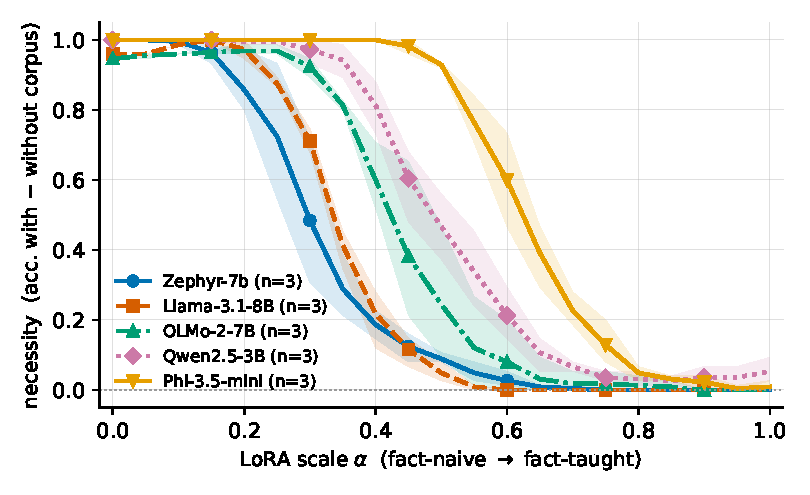
\includegraphics[width=0.72\textwidth]{figures/factqa_dose.pdf}}{%
  \fbox{\parbox{0.68\textwidth}{\centering\vspace{1.5em}\itshape figures/factqa\_dose.pdf --- generated
  by \texttt{experiments/unlearning/plot\_headline.py} from the headline run
  (\texttt{experiments/colab\_headline.ipynb}); this slot fills automatically once the PDF is
  committed.\vspace{1.5em}}}}
\caption{The fact-QA necessity dose-response (companion to Table~\ref{tab:dose}): necessity (accuracy
with $-$ without corpus) vs.\ LoRA-$\alpha$ on the dense 21-point grid, one line per model family,
shaded bands the min--max across three seeds. Five independent lineages collapse to a $\le\!0.05$ floor with knees at
five different $\alpha$---the known-groups calibration that makes a near-zero necessity reading
trustworthy.}
\label{fig:factqa_dose}
\end{figure}

\begin{table}[t]
\centering\small
\begin{tabular}{@{}lccccc@{}}
\toprule
& $\alpha{=}0$ & $0.25$ & $0.5$ & $0.75$ & $\alpha{=}1$ \\
\midrule
Zephyr-7B      & $1.00$ & $0.72$ & $0.09$ & $0.00$ & $0.00$ \\
Llama-3.1-8B   & $0.96$ & $0.88$ & $0.05$ & $0.00$ & $0.00$ \\
OLMo-2-7B      & $0.95$ & $0.97$ & $0.24$ & $0.02$ & $0.00$ \\
Qwen2.5-3B     & $1.00$ & $1.00$ & $0.47$ & $0.04$ & $0.05$ \\
Phi-3.5-mini   & $1.00$ & $1.00$ & $0.93$ & $0.13$ & $0.01$ \\
\bottomrule
\end{tabular}
\caption{Necessity dose-response by construction (the calibration): mean necessity over three seeds at
a subset of the 21-point LoRA-$\alpha$ grid (the full grid is plotted in Figure~\ref{fig:factqa_dose};
rows ordered by knee). All five families collapse to a $\le\!0.05$ floor, with knees at five different
$\alpha$. Seeds are monotone through the transition ($\le\!0.04$ per-step wiggles at the floor only);
the sub-$1.00$ starts for Llama and OLMo are the base models guessing a probe closed-book,
consistently across seeds.
The answer-accuracy objective uses no simulator. The decision-based hazard
domain does \emph{not} yield such a curve---teaching the fact as prose leaves the scored maneuver
unmoved (the \emph{knowing\,$\neq$\,doing} gap of Section~\ref{sec:necessity}); it is reported there,
not as a second calibration.}
\label{tab:dose}
\end{table}

\section{The corpus diagnosis}
\label{sec:diagnosis}
The calibrated necessity measure is the input to a per-item \emph{corpus diagnosis}: run the
different$\times$usable reading (Figure~\ref{fig:diffbetter}) on every item and label it. The three
non-relied cells demand different fixes. An \emph{unchanged} decision that succeeds is \textbf{redundant}
(the model already knows it; prune it), calibrated against the dose-response floor
(Section~\ref{sec:necessity}) so a near-zero reading means already-known rather than never-used. An
unchanged decision that fails is \textbf{ignored}/\emph{unusable} (present but the model cannot execute
it). The remaining cell is the sharp one.

\paragraph{The misled result.} The top-right cell of Figure~\ref{fig:diffbetter}---the decision
\emph{changes} but still \emph{fails}---is where a learner faithfully follows a \emph{wrong} retrieved
rule. This is the failure the whole measure is built to expose. Consider a corpus item that instructs
the wrong give-way maneuver. A faithful learner applies it, and when the item is ablated the learner
falls back on a safer parametric reflex and clears---so the item's raw necessity is \emph{maximal}: the
decision swings hard, exactly the signature of strong reliance. Yet the outcome \emph{with} the item is
a grounding. A subtractive necessity test (``did removing it hurt?'') and an influence-based
faithfulness score both report this item as heavily used and well-grounded---they cannot distinguish a
learner relying on a correct rule from one faithfully executing a harmful one, because both change the
output and both are ``supported'' by the context. The two-observable reading separates them: the
misled item lands in the top-right cell (changes the call, fails with it), never in \textbf{relied}
(top-left). The instrument's diagnostic value is precisely that faithful compliance with a wrong rule
is worse than ignoring it, and only the succeeds-with observable can see the difference.

\paragraph{The learners that exercise the override.} Necessity is always measured against a
\emph{learner}, and the misled/override contrast needs a cast that varies in how deeply it uses the
corpus: a \textbf{blind} learner cannot perceive the danger and collides; a \textbf{naive} learner is
sighted but untrained and avoids generically; an \textbf{implementer} applies a corpus rule verbatim
where the situation matches; and a \textbf{reasoner} treats the corpus as premises and combines it with
base rules for novel cases. On a matched suite where the textbook rule already fits, implementer and
reasoner are indistinguishable ($\Delta$regret $0.00$); on a conflict suite built so the safe side
\emph{alternates} port/starboard---so no fixed reflex passes---the reasoner clears $6/6$ while the
lookup implementer clears only the $3$ reaches where the local rule is redundant with Rule~14 and
\emph{grounds on the $3$ it overrides}. The necessity of the local-rule corpus is thus $3/6$, separable
\emph{only} on the overriding cases: this is the RAG-as-lookup vs.\ RAG-as-reasoning-substrate
distinction made measurable, and it is exactly the axis on which a \emph{wrong} local rule produces the
misled failure above (an implementer follows it off the cliff; the two-observable reading catches the
result). A live model run confirms the reading is not an artifact of hand-built policies:
Gemini-2.5-flash applies the local rule like a reasoner, relying on it on all three override reaches
($5/5$ samples, necessity $1782\pm0$)---with the corpus it alters to port and clears, ablated it applies
Rule~14 and grounds.

\paragraph{The misled result on a real model.} The same live model, run through a \emph{misled} arm---a
corpus rule that instructs the wrong (port) give-way toward an \emph{observable} obstacle, so following it
grounds while the ablated model clears---makes the blind spot empirical rather than hypothetical. Over four
misled scenarios $\times$ six samples (temp-$0$ point $+$ $K{=}5$ at $0.7$; $n{=}24$ draws per condition),
Gemini's harmful into-the-obstacle maneuver rate rises from $\mathbf{4\%}$ ablated to $\mathbf{33\%}$ with
the wrong rule, while its correct give-way rate falls from $70\%$ to $33\%$---the corpus roughly $8\times$'s
the harmful action and halves the correct one. Read per sample as a binary cell the signal is noisy (misled
on $1.6/4$ cells on average); read as the \emph{marginal maneuver rate} it is a clean, large shift, and the
marginal rate is what we report. The mechanism is not a perception failure---ablated, the model almost never
turns toward the obstacle ($1/24$ draws) and correctly cites it---but a \emph{confabulation}: with the wrong
rule present it turns toward the obstacle and reports that doing so ``passes clear of the moored barge.'' So
the model that applies \emph{correct} local rules like a reasoner (above) is, on \emph{wrong} ones, a
rule-follower whose harmful compliance a standard necessity or faithfulness score would credit as high,
well-grounded reliance---exactly the case the succeeds-with observable is built to catch. We report this as
a single-model effect size and its mechanism, not a rate we generalize.

\paragraph{Offline recovery of known ground truth.} Before any real-model sweep we confirm the
classification recovers truth we control. Against two reference mock learners the instrument is exact:
the corpus-bound mock's decision \emph{changes} on ablation and it then grounds (regret $0.2$ with the
rule $\to 1981$ without $\Rightarrow$ \emph{relied}); the leaking mock's decision is \emph{unchanged}
and clears both ways ($\Rightarrow$ \emph{redundant}). The whole offline backbone regenerates in one
deterministic, LLM-free command that checks each headline result against its claimed value.

\paragraph{A supporting cross-model reading (demoted).} As one supporting breadth result we run the
necessity test as a suite of eight independent, alternating-bow charted hazards, each isolated in its
own corpus, so per-model necessity is the fraction of the suite relied upon
(Table~\ref{tab:disc}). This gives a graded reliance spectrum across five production models, but the
counts must be read with an important caveat: they reflect ablated-arm fallback as well as reading. The
suite is $4$ override reaches (the hazard sits where the default Rule-14 starboard turn grounds) plus
$4$ where starboard already clears, so a model that falls back on the starboard reflex when the rule is
ablated is \emph{rescued} on the four non-override reaches and caps at $4/8$ \emph{by construction}.
Claude Opus's $8/8$ is co-determined by this: it \emph{holds course} when ablated (strict-mode
faithfulness---``no rules were provided'') rather than falling back on Rule-14, so it grounds on all
eight, whereas reflex-appliers like Haiku ($4$) cap at four by construction. Opus's $8/8$ therefore
means it does not fall back, not that it out-reads Haiku; the spectrum grades reading and ablated-arm
conservatism together, which is why we demote it to support rather than headline.

\begin{table}[t]
\centering
\small
\begin{tabular}{@{}lccc@{}}
\toprule
Model & relied & unusable & redundant \\
\midrule
Claude Opus 4.5      & $\mathbf{8}$   & $0$            & $0$ \\
Claude Haiku 4.5     & $4$            & $0$            & $4$ \\
Claude Sonnet 4.5    & $3$            & $2^{\dagger}$  & $3$ \\
Amazon Nova-micro    & $2^{\dagger}$  & $2^{\dagger}$  & $4$ \\
Llama-4-Maverick-17B & $0$            & $4$            & $4$ \\
\bottomrule
\end{tabular}
\caption{Cross-model necessity over the eight-hazard corpus-only suite (five models, AWS Bedrock).
Each hazard is isolated in its own corpus, so the three counts partition the suite of $8$ and per-model
reliance is a fraction. Classification uses \emph{necessity}
$=\regret(\text{ablated})-\regret(\text{with-corpus})$ and \emph{regret-with}: \textbf{relied} $=$
necessity $>100$ \emph{and} regret-with $<10$; \textbf{unusable} $=$ regret-with $\ge 10$ (grounds
\emph{with} the item present); \textbf{redundant} $=$ otherwise (clears both ways). Values are the
temp-$0$ point estimate; the $K{=}5$ temp-$0.7$ ensemble has sd $\approx\!0$ except ($\dagger$): Sonnet
unusable $1.2\pm0.7$, Nova-micro relied $0.2\pm0.4$ and unusable $2.2\pm0.7$. \textbf{Counts reflect
ablated-arm fallback as well as reading:} reflex-appliers cap at $4/8$ (the four override reaches), and
Opus's $8/8$ reflects that it holds course rather than falling back on Rule-14 when the rule is ablated.}
\label{tab:disc}
\end{table}

\paragraph{Per-rule attribution.} To show the diagnosis attributes reliance to a \emph{specific} rule
rather than to corpus presence in general, we add a second, independent rule (Rule~15 crossing
give-way) exercised on its own crossing scenarios. Ablating each rule produces a large regret signal on
its own encounters and localizes there: on \texttt{gemini-flash-latest}, ablating Rule~14 gives
$\delta_{\!\regret}{=}1981$ (head-on) and ablating Rule~15 gives $1285$ (crossing), each on its own
disjoint scenario subset, so the instrument reads reliance per rule, not merely per corpus.

\paragraph{Corpus sufficiency and \emph{false sufficiency}.} Rolling the per-item classifications to the
corpus level yields a sufficiency judgement for a query set: \emph{contributing} (every item relied
upon), \emph{partial}, \emph{unusable}, or---the diagnostic ordinary RAG metrics cannot produce---%
\emph{false sufficiency}: task accuracy is high yet necessity is $\approx\!0$ everywhere, so the corpus
is not carrying the load and success rides on priors, fragile to distribution shift. The claim is
explicitly scoped to the probed query set (sufficiency is always ``for these queries''); the
false-sufficiency signal is precisely the measurable warning that a bounded-query sufficiency claim
will not survive a shift. A finer presence-vs-retrieval decomposition is developed in
Appendix~\ref{app:retrieval}.

\section{Limitations and scope}
\label{sec:limits}
\textbf{Mechanism, not external validity.} Every result here is simulation-based mechanism evidence. We
make no learning-gains claim; the pre-registered human cohort study is the external-validity test this
in-silico screen is built to de-risk, and it is the endpoint, not a claim of this paper.
\textbf{Seed coverage.} The calibration dose-response is \emph{complete}: five families $\times$
three seeds $\times$ 21 grid points from a single clean run, every cell filled. The knowing\,$\neq$\,doing flat-hazard result is three-seed. What remains
single-seed (seed~$0$) is the pair of decision-domain \emph{follow-ups}: the CoT-elicitation bridge
($\approx\!0.3$ elicited) and the direct-install (decision-format SFT) arc, whose point values we treat
as single-run evidence, keeping the corresponding hedging in Section~\ref{sec:necessity}. Provenance
(per-seed CSVs and full per-fact audit logs) is in \texttt{experiments/provenance/dose-response/};
the offline mock recovery already confirms the \emph{instrument} recovers ground truth on these domains.
\textbf{Small evidence base.} The cross-model
reading (Table~\ref{tab:disc}) covers five models across three provider families on an eight-hazard
suite, and reflects ablated-arm fallback as much as reading (Section~\ref{sec:diagnosis}); it is a
worked example, not a leaderboard. \textbf{Decomposability may not generalize.}
\kc$\to$single-metric identifiability and clean per-rule ablation are properties we \emph{design into} a
governed corpus and \emph{verify} per instrument (Table~\ref{tab:ident}); an arbitrary corpus whose
rules are entangled may only support coarser, group-level attribution. \textbf{Which channel counts is a construct choice.} Necessity is read through a \emph{channel}---a
recalled fact or an executed decision---and the knowing\,$\neq$\,doing gap (Section~\ref{sec:necessity})
shows the two can diverge: a fact the model demonstrably holds (recall rises $0.00\!\to\!0.78$) can
leave a single-shot decision unmoved. The valid channel is therefore a property of the downstream
question, not of the instrument. For a corpus-bounded \emph{tutor}, whose target is what the learner
comes to \emph{know}, the recall/knowledge channel (our fictional-fact calibration) is the faithful
proxy, and reading necessity off an un-elicited decision would wrongly score an acquired fact as
\emph{unnecessary}; for a corpus-bounded \emph{agent} that must act, only the decision counts and a
knowing-but-not-doing fact is a genuine failure the recall channel would miss. An instrument should
declare its target construct and, where application matters (procedural knowledge, \citealp{koedinger2012kli}),
elicit before scoring or measure both channels and treat their gap as diagnostic rather than noise.
\textbf{Proxy validity.}
Simulated learners can be unfaithful; recent work documents systematic LLM-vs-human fidelity gaps
\citep{validsim2026,studentfidelity2025,studentabilities2025}, which is another reason the human study,
not the screen, is the endpoint.

\section{Conclusion}
\label{sec:conclusion}
We described an in-silico instrument that measures whether a learner \emph{needs} a corpus before any
human-subject effort, and made the measure trustworthy by \emph{constructing} its ground truth:
teaching many invented facts into a model's weights drives the instrument's necessity for them down as
a graded dose-response ($1.00$ to a $\le\!0.05$ floor across a 21-point gradient, in a simulator-free
QA domain, replicated across five model families at three seeds each, with knees at five different
points). A decision-based domain adds a validity caution the field should carry:
a fact taught as prose is recallable yet does not move a single-shot decision (a
\emph{knowing\,$\neq$\,doing} gap) unless reasoning \emph{elicits} it, so the necessity channel must
match the downstream construct. On that calibrated measure we built a corpus diagnosis whose sharpest
output is the \emph{misled} case---a learner faithfully following a wrong retrieved rule looks maximally
reliant yet is harmed, invisible to influence-based faithfulness and to subtractive necessity, and
caught only by reading necessity as decision-change \emph{and} succeeds-with. The claim is testable and
narrow, the domains are worked examples, and the measurement method---calibrated, and honest about
being a pre-human-study screen---is the point.

\section*{Reproducibility statement}
Every result here is simulation-based, and the pipeline is built to regenerate deterministically. The
offline backbone---construct validity and grading (Table~\ref{tab:construct}),
\kc$\to$single-metric identifiability (Table~\ref{tab:ident}), the offline mock recovery
(Section~\ref{sec:diagnosis}), and estimator recovery (Appendix~\ref{app:recovery})---rebuilds from a
single LLM-free command, and each headline value is checked against its claimed number in that run. The
GPU dose-response experiments (teach $+$ LoRA-$\alpha$ and checkpoint sweeps, both the fictional-fact
calibration and the decision-domain follow-ups) are driven by a single submittable job
(\texttt{experiments/gpu\_job.sh}: LoRA SFT teach, then a one-load generation sweep over the 21-point
$\alpha$ grid against a pre-committed prompt set) over pinned model identifiers
(\texttt{Qwen2.5-3B-Instruct}, \texttt{Phi-3.5-mini-instruct}, \texttt{zephyr-7b-beta},
\texttt{Llama-3.1-8B-Instruct}, and \texttt{OLMo-2-1124-7B-Instruct} for the reported calibration;
\texttt{Qwen2.5-3B-Instruct} for the decision domain), seeds $\{0,1,2\}$ per family (the
decision-domain follow-ups are seed~$0$), and the LoRA and SFT hyperparameters reported inline in
Section~\ref{sec:necessity}. Calibration generation is batched greedy decoding guarded by a per-job
batched-vs-single-stream self-check that falls back to single-stream on mismatch.
All scoring is replayed off-GPU from the saved per-$\alpha$ transcripts;
the per-seed CSVs and full per-fact audit logs behind every calibration number are committed under
\texttt{experiments/provenance/dose-response/}. Live-model results
(Section~\ref{sec:diagnosis}) are reported as single-model effect sizes with the exact prompts,
temperatures, and sample counts stated, and are not generalized; because hosted APIs can drift, these
are the one component not bit-reproducible. All corpora, teach sets, drivers, and provenance logs are
included in the anonymized supplementary material and will be released in a public repository on
acceptance.

\appendix

\section{The categorical leakage verdict (secondary)}
\label{app:verdict}
The main text classifies each item on two observables---does the decision change on ablation, and does
the learner succeed with the item present (Figure~\ref{fig:diffbetter}). For continuity with prior
leakage work we also compute a coarser \emph{categorical} verdict,
\textsc{corpus-bound}/\textsc{leaking}/\textsc{inconclusive}, by a majority vote over three signals:
the ablation-delta (does regret rise when the rule is removed), a \emph{counterfactual} test (replace
``alter to starboard'' with ``alter to port''---does the learner follow the altered rule?), and a
\emph{closed-book} contamination baseline (no corpus supplied). The majority vote keeps a single
dissenting sub-test from vetoing a clear ablation-and-contamination pattern. We de-emphasize it because
it is noisier than the two continuous observables and \emph{undercounts} a model whose decision plainly
depends on the fact but which answers closed-book from priors---it put Haiku at $0/8$ where the
decision-change reading gives $4/8$.

\paragraph{Strict-mode reading on standard COLREG.} The verdict is retained mainly for one signal it
reads cleanly. On \emph{standard} COLREG, Claude Opus verdicts \textsc{corpus-bound}, but the audit log
shows this is strict-mode faithfulness, not a knowledge gap: when the steering rule is ablated Opus
abstains/holds course (``no rules were provided\ldots'') rather than falling back on its obvious
parametric Rule-14, while Haiku falls back to Rule-14 starboard (\textsc{leaking}) and Sonnet splits
across samples (\textsc{inconclusive}). This is the same ablated-arm behavior that co-determines Opus's
$8/8$ in Table~\ref{tab:disc}.

\section{Validation by unlearning: a \emph{says\,$\neq$\,does} dissociation}
\label{app:unlearning}
The complementary weight-level direction removes a rule the model \emph{does} know and asks whether
necessity rises. This arm is secondary---it has dynamic range only on a rule with a real
corpus-vs-prior gap, which the standard rules lack---but it yields an independently interesting result.
We remove the alter-to-starboard knowledge from an open-weight model with a real unlearning
method---SimNPO \citep{simnpo2024} as primary (reference-free, length-normalized), with NPO
\citep{npo2024}, RMU \citep{rmu2024}, and gradient ascent \citep{ga2023} as baselines---and score the
base vs.\ unlearned model on the reference-policy instrument. A removal audit \citep{lynch2024} reports
whether the knowledge is \emph{gone} vs.\ merely \emph{suppressed}; for a stable novice that resists
benign relearning we layer in a robust utility-preserving recipe \citep{unlearninglasts2025}. A
completed GPU run (gentle, guardrailed SimNPO on Qwen2.5-3B; config in Table~\ref{tab:unlearn})
delivers a lesson sharper than the predicted $2\times2$: \textbf{standard free-text unlearning metrics
overstate removal because they measure what the model \emph{says}; the reference-policy instrument
measures what the model \emph{does}---its steering decision---and shows the decision is untouched.}

\paragraph{Primary result: a \emph{says\,$\neq$\,does} dissociation.} Every metric that reads the
model's \emph{words} registers forgetting: on the GPU run the forget-probe ``starboard'' rate falls
$0.43\to0.27$, the forget-set NLL rises $7.4\to32.4$ (retain-set NLL, teacher-forced, even
\emph{improves} $4.3\to1.07$), and---most tellingly---the Rule-14 \emph{citation} disappears, the model
reattributing its maneuver to Rules 15/16/17. (A CPU run reproduces the likelihood collapse
method-agnostically: forget NLL $4.6\to92$, direction-cue $5/6\to0/6$.) Yet the \emph{decision} the
instrument scores does not budge: the unlearned model's completions \emph{still turn $+30^\circ$ to
starboard} (model damage flat at $0.10$, retain-coherence $0.91$). A words-level metric reports a fact
removed while the policy that governs behavior is entirely intact.

\paragraph{Suppressed, not removed; and the aggressive inversion.} Twenty benign fine-tuning steps pull
the forget-set NLL $32.4\to9.2$, back near its base value---the textbook suppressed-not-removed
signature. By contrast an earlier aggressive recipe (lr $1\!\times\!10^{-4}$, no guardrail) drove model
damage $0.10\to0.33$ and turned the ship to \emph{port}---the wrong way---on $6/8$ prompts: because the
head-on turn is essentially binary, the default objective simply relocated the mass onto ``port,''
\emph{inverting} the safety rule, a caution that naive weight-level unlearning of a safety rule can
yield confident non-compliance. \textbf{Why the $2\times2$ is flat:} Rule~14 already \textsc{leaks} at
baseline---every frontier model knows head-on\,$\to$\,starboard parametrically---so ablating it changes
nothing (ablation-delta $0$), leaving no dynamic range. The \textsc{leaking} verdicts are therefore
\emph{correct}; this is exactly why the primary weight-level validation is the construction
dose-response (Section~\ref{sec:necessity}), where a corpus-only fact \emph{does} have range.

\begin{table}[h]
\centering
\small
\begin{tabular}{@{}lcccc@{}}
\toprule
 & \multicolumn{2}{c}{1.5B (CPU, SimNPO)} & \multicolumn{2}{c}{3B (GPU, gentle SimNPO)} \\
\cmidrule(lr){2-3}\cmidrule(lr){4-5}
Metric & base & unlearned & base & unlearned \\
\midrule
Forget-target NLL ($\uparrow$)              & 4.6 & 92.0 & 7.4  & 32.4 \\
Retain-set NLL, teacher-forced ($\downarrow$)& 3.2 & 0.18 & 4.3  & 1.07 \\
Forget-probe ``starboard'' rate ($\downarrow$)& 5/6 & 0/6 & 0.43 & 0.27 \\
Retain-coherence, free-gen ($\uparrow$)     & --- & ---  & 1.00 & 0.91 \\
Model damage (wrong+degen., $\downarrow$)   & --- & ---  & 0.10 & 0.10 \\
\emph{Steering decision (instrument)}       & --- & ---  & \emph{stbd} & \emph{stbd} \\
\bottomrule
\end{tabular}
\caption{Gentle, guardrailed SimNPO unlearning of the alter-to-starboard rule, on a 1.5B model (CPU)
and Qwen2.5-3B (GPU, \texttt{bfloat16}; lr $5\!\times\!10^{-5}$, retain\_weight $3.0$, Rule-14 kept in
the retain set). Every \emph{words-level} metric registers forgetting while retain utility is preserved
and there is no inversion (model damage flat at $0.10$). Yet the \emph{decision} the instrument scores
is untouched: the unlearned model still turns $+30^\circ$ to starboard, and the $2\times2$ stays verdict
\textup{\textsc{leaking}}, ablation-delta $0.000$---a says\,$\neq$\,does dissociation. Benign relearning
($20$ steps) pulls forget NLL $32.4\to9.2$, confirming the fact was \emph{suppressed}, not removed.}
\label{tab:unlearn}
\end{table}

\section{Estimator recovery and calibration}
\label{app:recovery}
Feeding the instrument's outcomes into a generic learner-agent estimator, we recover known ground truth
on synthetic data (Table~\ref{tab:recovery}). This turns ``we have a metric'' into ``the measurement is
valid.''

\begin{table}[h]
\centering
\small
\begin{tabular}{@{}lll@{}}
\toprule
Estimator & Recovery of known ground truth & Calibration (ECE) \\
\midrule
Elo & static ability, mean abs.\ error $0.046$ & $0.023$ \\
BKT & latent state $P(\hat L)=0.997$ (learned) vs.\ $0.175$ (not) & $0.004$ \\
\bottomrule
\end{tabular}
\caption{Estimator-recovery and calibration on synthetic data with a known ground truth. The
measurement, not just the metric, is validated.}
\label{tab:recovery}
\end{table}

\section{Presence vs.\ retrieval: what in the corpus changes the answer}
\label{app:retrieval}
The necessity test asks whether the learner relies on the corpus \emph{at all}; a deployed RAG tutor
raises a finer question---of the value curation adds, how much comes from the fact being \emph{present}
versus the retriever actually \emph{surfacing} it. Decomposing over in-corpus $\times$ retrieved gives
three scorable conditions: \textsc{none} (closed-book, priors only), \textsc{retrieved} (the deployed
dense retriever's top-$k$), and \textsc{oracle} (the answer-bearing chunk, i.e.\ perfect retrieval).
Accuracy across them attributes the gain: $\mathrm{acc}(\textsc{oracle}){-}\mathrm{acc}(\textsc{none})$
is the \emph{content ceiling}, $\mathrm{acc}(\textsc{retrieved}){-}\mathrm{acc}(\textsc{none})$ is what
the deployed pipeline \emph{delivers}, and their difference is the \emph{retrieval gap}. On seven
equipment-SOP fact-recall queries through a small local generator (Qwen2.5-1.5B), closed-book accuracy
is $0/7$, \textsc{oracle} is $7/7$, and the deployed MiniLM pipeline lands between at $3/7$---so of a
$100\%$ content ceiling the pipeline \emph{delivers} $43\%$ and \emph{forfeits} a $57\%$ retrieval gap.
A curation failure (fact absent), a retrieval failure (present but unranked), and a priors success are
distinct outcomes the binary leakage verdict cannot separate. (Numbers illustrate the method---one
small model, seven queries---not a benchmark.)

\small
\bibliographystyle{tmlr}
\bibliography{refs}

\end{document}
